\section{Auswertung}
Im Folgenden werden die Messungen präsentiert und nötige Rechnungen durchgeführt. Zunächst
werden die Kalibrierungen der lateralen Position vorgestellt, mit denen aus einem Spannungssignal der
Viersegment Diode eine Position auf der Probe angegeben werden kann. Dies wird genutzt um anschließend
aus den Messungen an den Quarzkugeln und Polysterenkugeln die Boltzmann-Konstante, sowie die leistungsabhängige
Fallensteifigkeit zu bestimmen. Abschließend werden die Messungen und Beobachtungen an den Zwiebelzellen
gezeigt.

\subsection{Kalibrierung der lateralen Position}
Die Daten der Kalibrierung der lateralen Position konnten nicht aus der Thorlabs-Software extrahiert werden. Zwei
Kurven für den Verlauf der Diodenspannung beim räumlichen Scan über eine fixierte Quarzkugel sind in Abbildung~\ref{fig: calibration}
in einem Screenshot einzusehen. Anhand der grün eingefärbten linearen Regressionen an die Daten kann für alle Stromstärken eine
Umrechnung zwischen Spannung und Position ermittelt werden. Die einzelnen Umrechnungsfaktoren sind in Tabelle~\ref{tab: zcalibration} aufgeführt.

\begin{figure}
  \centering
  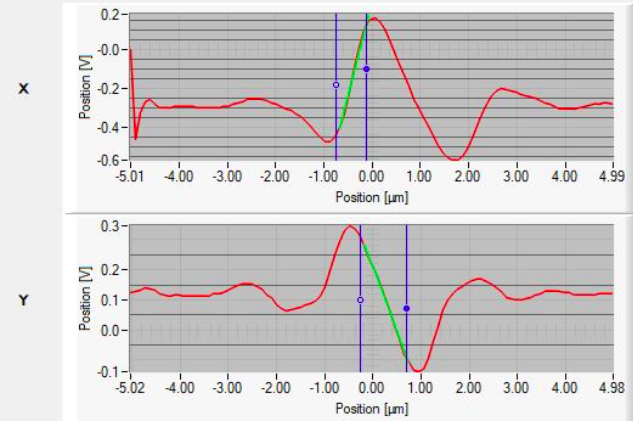
\includegraphics[width = 0.6\textwidth]{../analysis/data/i_quarz/70mA/position_calibration_70mA.png}
  \caption{Screenshot aus der Thorlabs Software. Die Kurven zeigen den Verlauf der Photodiodenspannung beim Scan über
  eine fixierte Quarzkugel. Die linearen, grün markierten Bereiche werden zur Kalibrierung zwischen lateraler Position und Spannung verwendet.}
  \label{fig: calibration}
\end{figure}
\begin{table}
	\centering
	\caption{Umrechnungsfaktoren zwischen Spannung der Viersegmentdiode und Strecke für die verwendeten Pumpströme.}
	\label{tab: zcalibration}
	\begin{tabular}{
		S[table-format=3.0]
		S[table-format=1.3]
		S[table-format=1.3]
		}
	\toprule
		{$I$\;/\;\si{\milli\ampere}} &
		{$s_x$\;/\;\si{\volt\per\micro\meter}} &
		{$s_y$\;/\;\si{\volt\per\micro\meter}} \\
	\midrule
		 70 &  0.963 & -0.439 \\
		 170 &  0.865 & -0.264 \\
		 270 &  0.759 & -0.157 \\
		 370 &  0.701 & -0.155 \\
		 470 &  0.727 & -0.152 \\
	\bottomrule
	\end{tabular}
\end{table}

\FloatBarrier
\subsection{Quarzkugeln}
Die Messungen an den Quarzkugeln wurden für die Pumpstromstärken $\SI{70}{\milli\ampere}$, $\SI{170}{\milli\ampere}$,
$\SI{270}{\milli\ampere}$, $\SI{370}{\milli\ampere}$ und $\SI{470}{\milli\ampere}$ durchgeführt. Da das Vorgehen der Auswertung
jeweils völlig analog funktioniert, werden hier nur im Detail die Messungen für $I = \SI{70}{\milli\ampere}$ gezeigt.
In Abbildung~\ref{fig: quarz_screenshot} ist eine eingefangen Quarzkugel gezeigt. Der gelbe Kreis gibt die Position
der optischen Pinzette an. Es ist anzumerken, dass nicht für alle Stromstärken die selbe Quarzkugel verwendet werden
konnte, da weitere Quarzkugeln in die Falle eingefangen wurden.
\begin{figure}
  \centering
  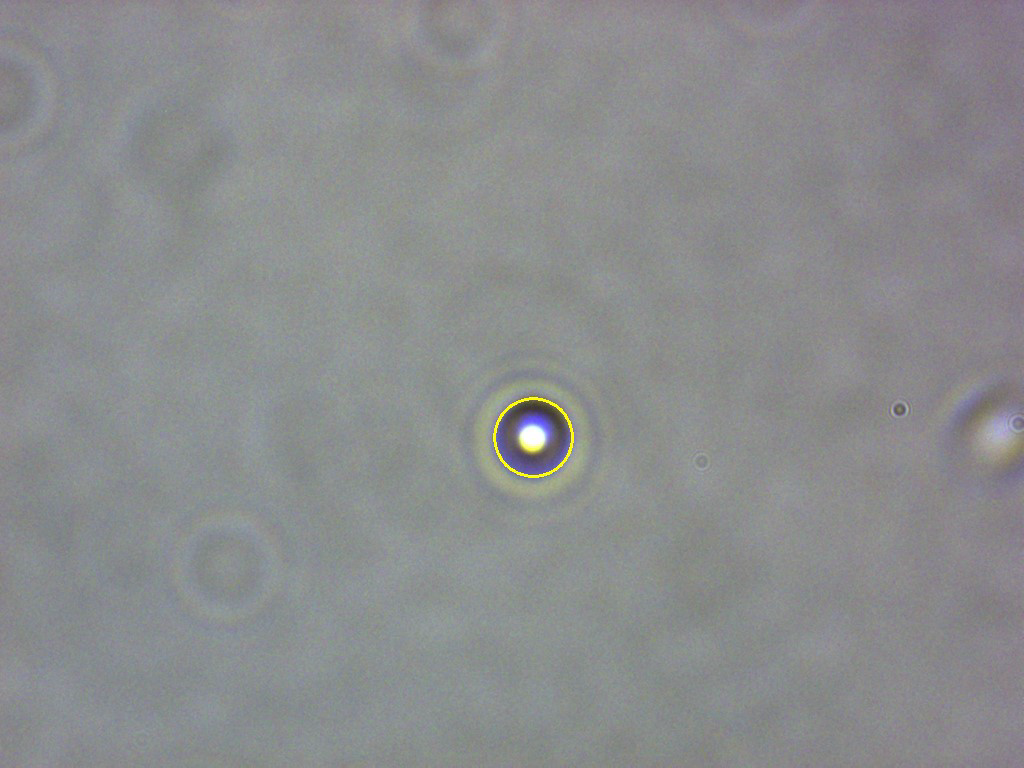
\includegraphics[width = 0.4\textwidth]{../analysis/data/i_quarz/70mA/070mA_screenshot.png}
  \caption{Bild einer eingefangen Quarzkugel mit einer Pumpstromstärke von $\SI{70}{\milli\ampere}$. Der gelbe Kreis gibt die
  Position der optischen Pinzette an.}
  \label{fig: quarz_screenshot}
\end{figure}
\FloatBarrier

Abbildung~\ref{fig: quarz_without_force}~(a) und (c) zeigen die Kugelpositionen in $x$- und $y$-Richtung ohne Einwirkung
einer Kraft. %(Amplitude $\SI{1}{\micro\meter}$, Frequenz $\SI{1}{\hertz}$) durch die Piezosteuerung des Probentisches.
Aus diesen Daten wird als Schätzer für die spektrale Leistungsdichte
ein Periodogramm berechnet. Dies ist jeweils in den Abbildungen~\ref{fig: quarz_without_force}~(b) und (d) einzusehen. Die Kurven werden
an eine Funktion der Gestalt
\begin{equation}
  PSD(f) = \frac{A}{f^2 + f_0^2}
  \label{eq: lorentz}
\end{equation}
angepasst. Hierin ist $f_0$ die \emph{roll-off}-Frequenz. Es ergibt sich
\begin{equation}
  f_{0, x} \approx \SI{4.0}{\hertz}, \quad f_{0, y} \approx \SI{5.4}{\hertz}.
\end{equation}
Aus diesen Frequenzen kann gemäß
\begin{equation}
  k = 2\pi \beta f_0
\end{equation}
die Fallensteifigkeit $k$ ermittelt werden. Abbildung~\ref{fig: quarz_k_power_series} zeigt die Abhängigkeit der Fallensteifigkeit von dem
Pumpstrom $I$ und damit von der Laser-Intensität. Die Datenpunkte sind in Tabelle~\ref{tab: quarz_result} eingetragen.
Es ist ein linearer Trend zu erkennen, wobei der Datenpunkt $k_x$
für $\SI{370}{\milli\ampere}$ deutlich ausreißt. Für die Steigungen $s$ ergeben sich aus einer linearen Regression
\begin{equation}
  s_x \approx \SI{0.8e-7}{\newton \per \meter \per \milli\ampere}, \quad  s_y \approx \SI{0.5e-7}{\newton \per \meter \per \milli\ampere}
\end{equation}
\begin{figure}
  \centering
  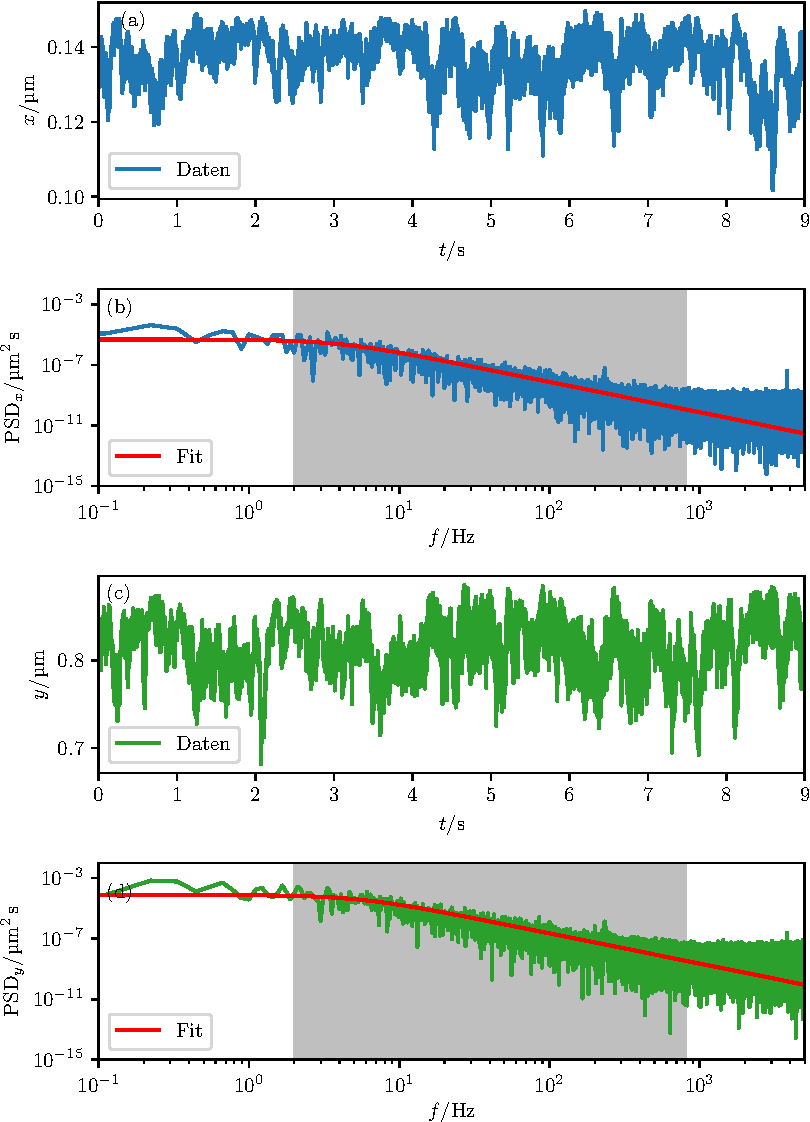
\includegraphics[scale = 1]{../analysis/data/i_quarz/70mA/results/without_force_70mA.pdf}
  \caption{Messreihe an den Quarzkugeln zur Bestimmung der \emph{roll-off}-Frequenz aus der zeitlichen Variation der Kugelposition ohne Einwirkung einer äußeren Kraft.
  (a) und (c) zeigen die Zeitserien für die $x$- bzw. $y$- Postion. (b) und (d) zeigen die berechneten spektralen Leistungsdichten und die Fits an das
  Modell~\eqref{eq: lorentz}. Für den Fit wurden nur die grau hinterlegten Daten verwendet.}
  \label{fig: quarz_without_force}
\end{figure}
\begin{figure}
  \centering
  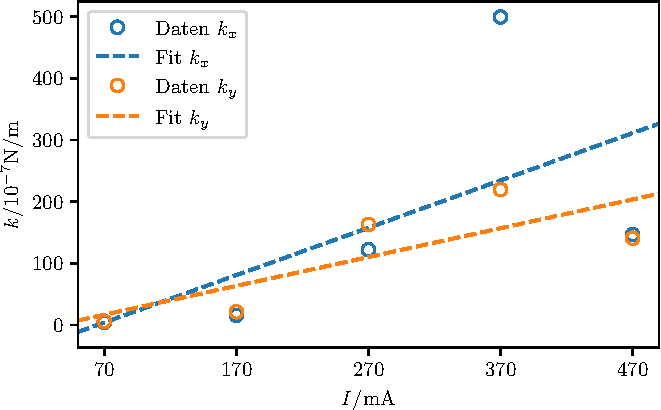
\includegraphics[scale = 1]{../analysis/data/i_quarz/k_power_series.pdf}
  \caption{Messreihe an den Quarzkugeln zur Untersuchung der Abhängigkeit der Fallensteifigkeit von dem Pumpstrom des Diodenlasers
  in $x$- und $y$-Richtung. Die Daten stammen aus der Messung ohne Krafteinfluss. }
  \label{fig: quarz_k_power_series}
\end{figure}

In den Abbildungen~\ref{fig: quarz_without_force}~(a) und~(c) ist
sowohl in $x$- als auch in $y$-Richtung eine Asymmetrie in der Verteilung der Positionen mit der Zeit zu erkennen.
Dies ist deutlicher in einer histogrammierten Ansicht (Abbildung~\ref{fig: quarz_without_force_hist}) zu beobachten.
Aus den Daten kann die Varianz $\langle x^2 \rangle \overset{\langle x \rangle = 0} = \langle x\rangle^2$ ermittelt werden
\begin{equation}
  \langle x^2 \rangle \approx \SI{4.1e-5}{\micro\meter\squared},\quad \langle y^2 \rangle \approx \SI{9.4e-4}{\micro\meter\squared}.
\end{equation}
Und hieraus unter Verwendung des Äquipartionstheorems Werte für die Boltzmann-Konstante
\begin{equation}
k_{B, x} \approx \SI{5.8e-26}{\joule\per\kelvin}, \quad k_{B, y} \approx \SI{1.8e-24}{\joule\per\kelvin}.
\end{equation}

Im Mittel aus allen Messreihen ergibt sich
\begin{equation}
  k_{B, mean} \approx \SI{39e-23}{\joule\per\kelvin}.
\end{equation}
Der seit diesem Jahr festgelegte Wert der Boltzmann-Konstante beträgt $\SI{1.380649e-23}{\joule\per\kelvin}$.
\begin{figure}
  \centering
  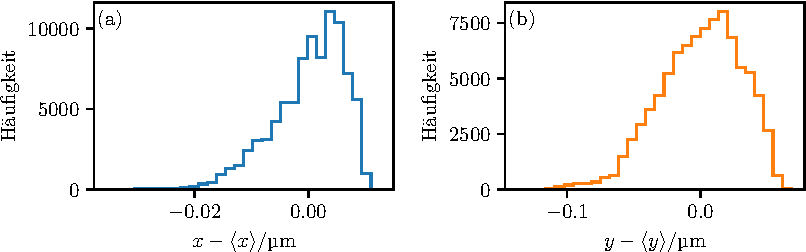
\includegraphics[scale = 1 ]{../analysis/data/i_quarz/70mA/results/without_force_histogram_70mA.pdf}
  \caption{Histogramme der Kugelpositionen aus der Messreihe in Abbildung~\ref{fig: quarz_without_force}.}
  \label{fig: quarz_without_force_hist}
\end{figure}

\FloatBarrier
Unabhängig von den Messungen ohne Krafteinwirkung
kann mit den Messreihen mit Krafteinwirkung erneut die Fallensteifigkeit untersucht werden. Abbildung~\ref{ig: quarz_with_force} zeigt die
Variation der Kugelpostion unter EInfluss einer periodischen Kraft (Amplitude $\SI{1}{\micro\meter}$, Frequenz
$\SI{1}{\hertz}$) durch die Piezosteuerung des Probentisches. Unter Verwendung des Kräftegleichgewichts
\begin{equation}
  k x = \beta v
\end{equation}
kann mit $v = \SI{2}{\micro\meter\per\second}$ die Fallensteifigkeit berechnet werden. Das Ergebnis der
Intensitätsabhängigen Messung ist in Abbildung~\ref{fig: quarz_k_power_series_force} dargestellt. Die Werte der Fallensteifigkeit sind in
Tabelle~\ref{tab: quarz_result}
eingetragen. Es zeigt sich eine deutliche Abweichung von einem linearen Anstieg. Auf eine weitere Analyse der Daten wird daher verzichtet.
Auf die Gründe für die fehlerhafte Messung wird in Kapitel~\ref{sec: diskussion} eingegangen.
\begin{figure}
  \centering
  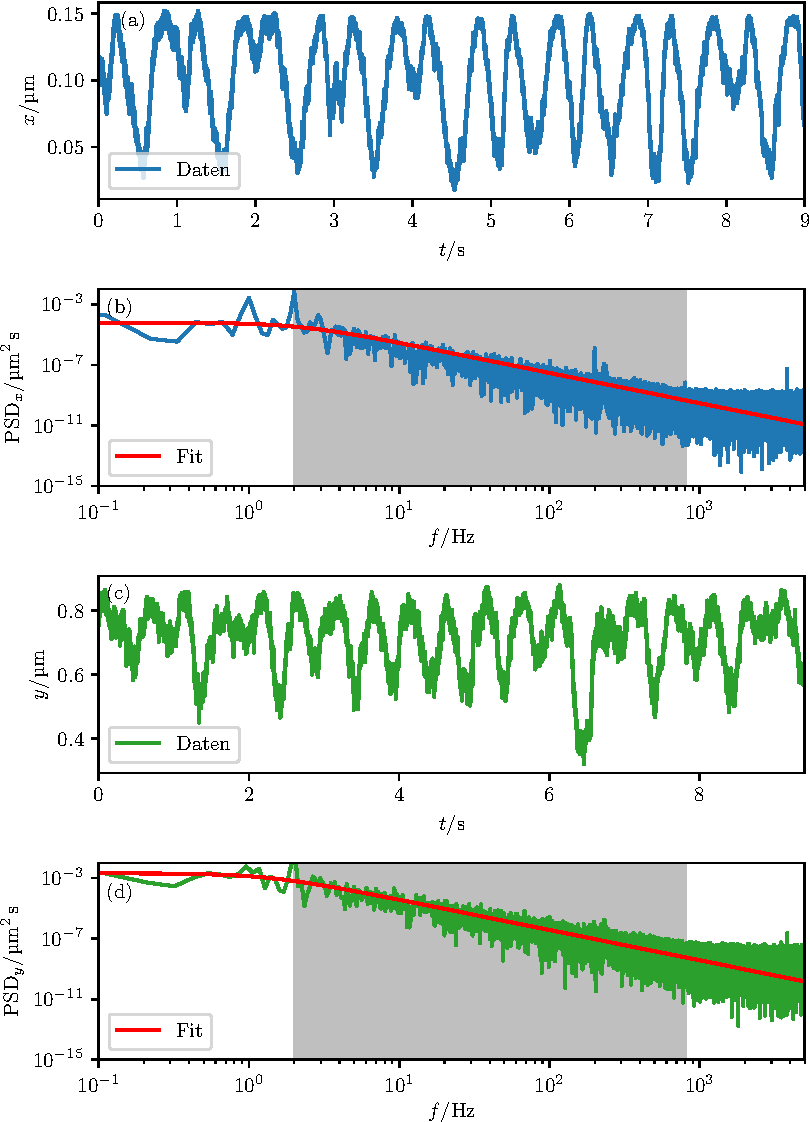
\includegraphics[scale = 1]{../analysis/data/i_quarz/70mA/results/with_force_70mA.pdf}
  \caption{Messreihe an den Quarzkugeln unter Einfluss einer äußeren Kraft zur Bestimmung der Fallensteifigkeit.  }
  \label{fig: quarz_with_force}
\end{figure}
\begin{figure}
  \centering
  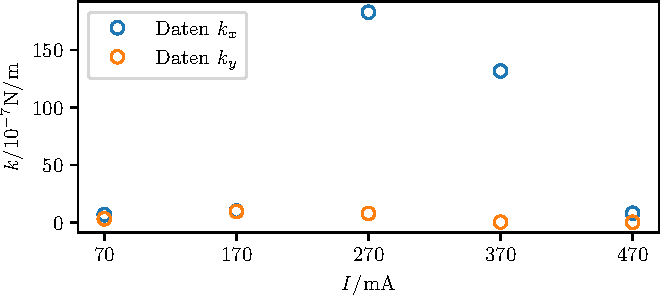
\includegraphics[scale = 1]{../analysis/data/i_quarz/k_power_series_force.pdf}
  \caption{Messreihe an den Quarzkugeln zur Untersuchung der Abhängigkeit der Fallensteifigkeit von dem Pumpstrom des Diodenlasers
  in $x$- und $y$-Richtung. Die Daten stammen aus der Messung mit Krafteinfluss. }
  \label{fig: quarz_k_power_series_force}
\end{figure}

\begin{table}
	\centering
	\caption{Ergebnisse für die Fallensteifigkeit in $x$- und $y$-Richtung. Die Ergebnisse wurden aus den Messungen ohne Krafteinwirkung sowie aus den Messungen mit Krafteinwirkung (Index F) gewonnen.}
	\label{tab: quarz_result}
	\begin{tabular}{
		S[table-format=3.0]
		S[table-format=3.1]
		S[table-format=3.1]
		S[table-format=3.1]
		S[table-format=3.1]
		}
	\toprule
		{$I$\;/\;\si{\milli\ampere}} &
		{$k_x$\;/\;\si{10^{-7}\newton\per\meter}} &
		{$k_y$\;/\;\si{10^{-7}\newton\per\meter}} &
		{$k_{x, F}$\;/\;\si{10^{-7}\newton\per\meter}} &
		{$k_{y, F}$\;/\;\si{10^{-7}\newton\per\meter}} \\
	\midrule
		 70 &  4.2 &  5.7 &  6.7 &  3.2 \\
		 170 &  15.5 &  21.1 &  10.0 &  9.5 \\
		 270 &  121.7 &  163.0 &  182.7 &  7.8 \\
		 370 &  499.3 &  219.3 &  131.7 &  0.3 \\
		 470 &  146.4 &  140.5 &  8.1 &  0.2 \\
	\bottomrule
	\end{tabular}
\end{table}

\FloatBarrier

\newpage
\subsection{Polysterenkugeln}
Analog zu der Auswertung aus dem vorangegenagen Abschnitt wird für die Polysterenkugeln vorgegangen.
Hier ist anzumerken, dass es hier, im Gegensatz zu den Messungen an den Quarzkugeln, gelungen ist, alle
Messungen an der selben Kugel durchzuführen.

Zum qualitativen Vergleich zwischen Quarz- und Polysteren-Probe ist für die
Stromstärke $\SI{70}{\milli\ampere}$ eine Messreihe ohne (Abbildung~\ref{fig: poly_without_force}) und
mit Krafteinwirkung (Abbildung~\ref{fig: poly_with_force}) dargestellt.
\begin{figure}
  \centering
  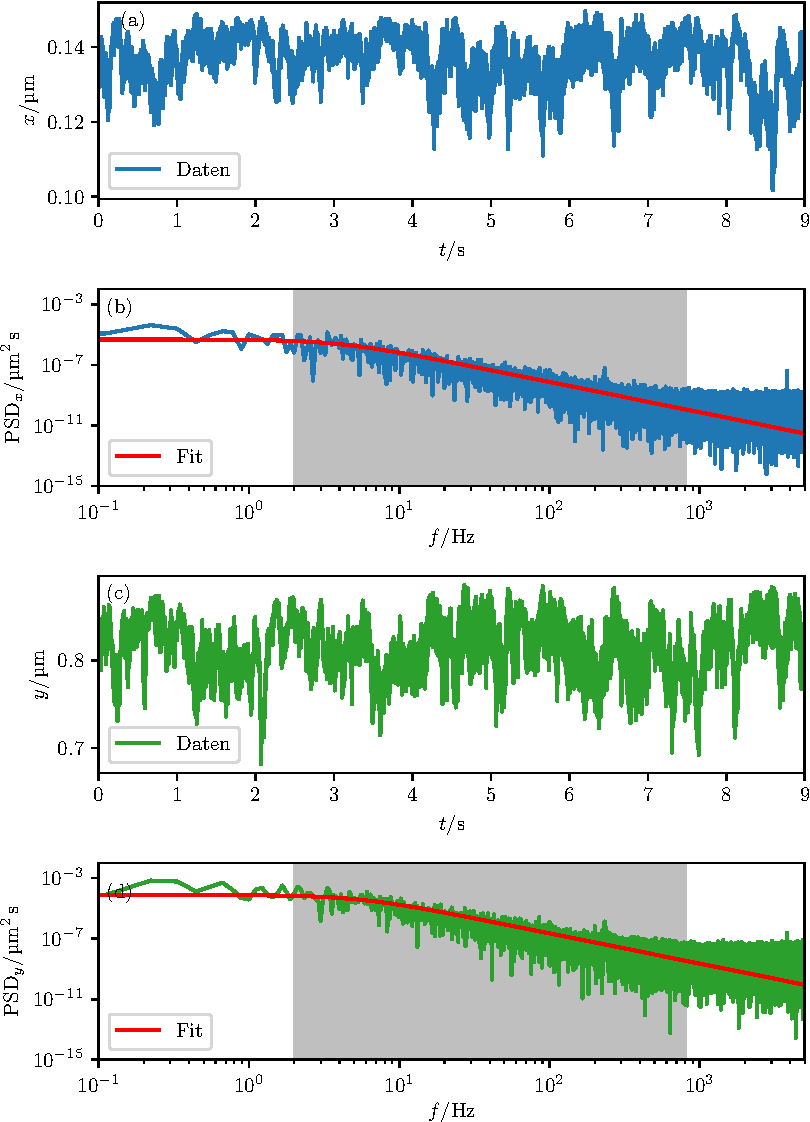
\includegraphics[scale = 1]{../analysis/data/i_quarz/70mA/results/without_force_70mA.pdf}
  \caption{Messreihe an den Polysterenkugeln zur Bestimmung der \emph{roll-off}-Frequenz aus der zeitlichen Variation der Kugelposition ohne Einwirkung einer äußeren Kraft.
  (a) und (c) zeigen die Zeitserien für die $x$- bzw. $y$- Postion. (b) und (d) zeigen die berechneten spektralen Leistungsdichten und die Fits an das
  Modell~\eqref{eq: lorentz}. Für den Fit wurden nur die grau hinterlegten Daten verwendet.}
  \label{fig: poly_without_force}
\end{figure}
\begin{figure}
  \centering
  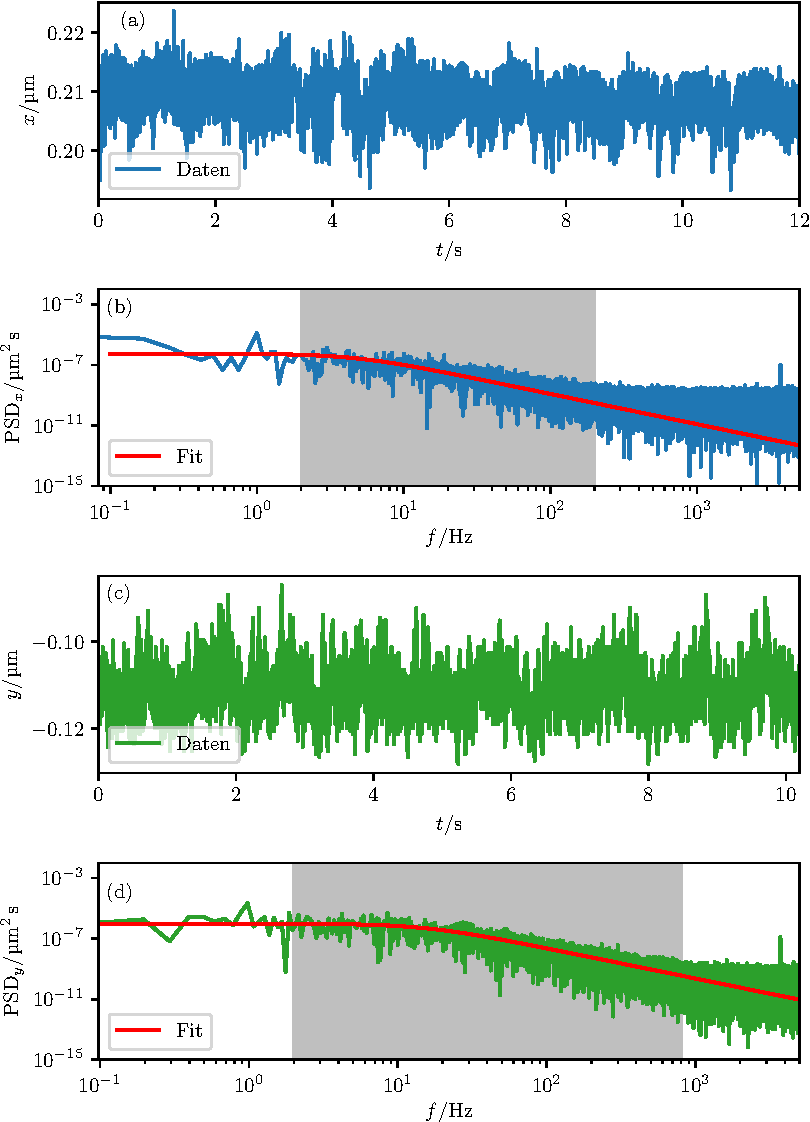
\includegraphics[scale = 1]{../analysis/data/ii_polysteren/70mA/results/with_force_70mA.pdf}
  \caption{Messreihe an den Polysterenkugeln unter Einfluss einer äußeren Kraft zur Bestimmung der Fallensteifigkeit.}
  \label{fig: poly_with_force}
\end{figure}

Abbildung~\ref{fig: poly_k_power} zeigt die Intensitätsabhängigkeit der Fallensteifigkeit aus der Messreihe ohne Krafteinwirkung,
Abbildung~\ref{fig: poly_k_power_series_force} zeigt den Verlauf aus der Messreihe mit Krafteinwirkung. Ale Werte sind in Tabelle~\ref{tab: poly_result}
eingetragen. Erneut ist ersichtlich, dass die Messung mit Krafteinwirkung keine Ergebnisse liefert.

Im Mittel aus allen
Messungen ohne Krafteinwirkung wird für die Boltzmann-Konstante der Wert
\begin{equation}
  k_B \approx \SI{6.1e-23}{\joule\per\kelvin}
\end{equation}
gefunden.

\begin{figure}
  \centering
  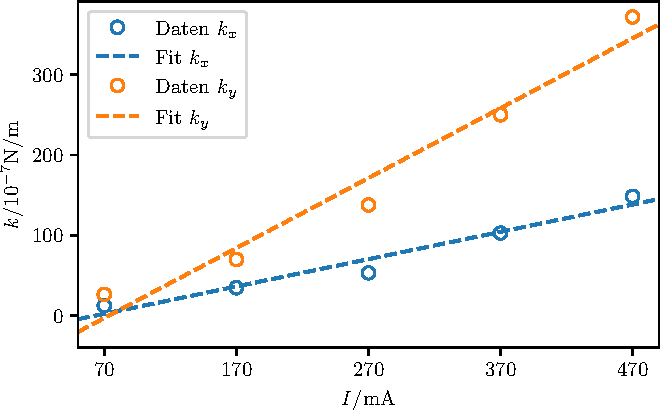
\includegraphics[scale = 1]{../analysis/data/ii_polysteren/k_power_series.pdf}
  \caption{Messreihe an den Polysterenkugeln zur Untersuchung der Abhängigkeit der Fallensteifigkeit von dem Pumpstrom des Diodenlasers
  in $x$- und $y$-Richtung. Die Daten stammen aus der Messung ohne Krafteinfluss.}
  \label{fig: poly_k_power}
\end{figure}
\begin{figure}
  \centering
  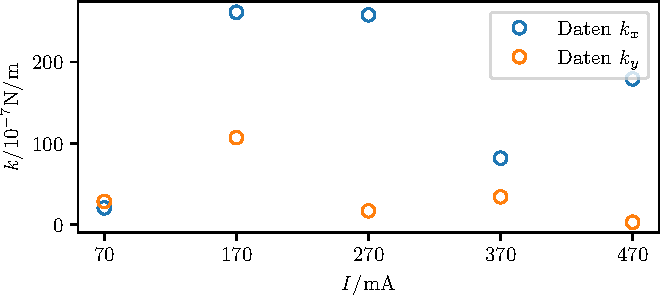
\includegraphics[scale = 1]{../analysis/data/ii_polysteren/k_power_series_force.pdf}
  \caption{Messreihe an den Polysterenkugeln zur Untersuchung der Abhängigkeit der Fallensteifigkeit von dem Pumpstrom des Diodenlasers
  in $x$- und $y$-Richtung. Die Daten stammen aus der Messung mit Krafteinfluss. }
  \label{fig: poly_k_power_series_force}
\end{figure}
\begin{table}
	\centering
	\caption{Ergebnisse für die Fallensteifigkeit in $x$- und $y$-Richtung. Die Ergebnisse wurden aus den Messungen ohne Krafteinwirkung sowie aus den Messungen mit Krafteinwirkung (Index F) gewonnen.}
	\label{tab: poly_result}
	\begin{tabular}{
		S[table-format=3.0]
		S[table-format=3.1]
		S[table-format=3.1]
		S[table-format=3.1]
		S[table-format=3.1]
		}
	\toprule
		{$I$\;/\;\si{\milli\ampere}} &
		{$k_x$\;/\;\si{10^{-7}\newton\per\meter}} &
		{$k_y$\;/\;\si{10^{-7}\newton\per\meter}} &
		{$k_{x, F}$\;/\;\si{10^{-7}\newton\per\meter}} &
		{$k_{y, F}$\;/\;\si{10^{-7}\newton\per\meter}} \\
	\midrule
		 70 &  12.2 &  26.2 &  20.6 &  28.5 \\
		 170 &  34.5 &  69.8 &  261.3 &  107.0 \\
		 270 &  53.0 &  137.7 &  258.1 &  17.0 \\
		 370 &  102.7 &  250.2 &  81.8 &  34.2 \\
		 470 &  148.4 &  372.0 &  179.3 &  2.9 \\
	\bottomrule
	\end{tabular}
\end{table}
\FloatBarrier

\subsection{Zwiebelzellen}
Nachfolgend werden die Beobachtungen an den Zwiebelzellen vorgestellt. Hierbei wird mehrfach auf Videos aus dem Anhang
verwiesen. Abbildung~\ref{fig: zwiebelzelle} zeigt zunächst eine exemplarische Aufnahme der Zwiebelzelle mit der CMOS-Kamera.
Mittig des Bildes sind die Vesikel innerhalb einer Mikrofaser deutlich zu erkennen.
\begin{figure}
  \centering
  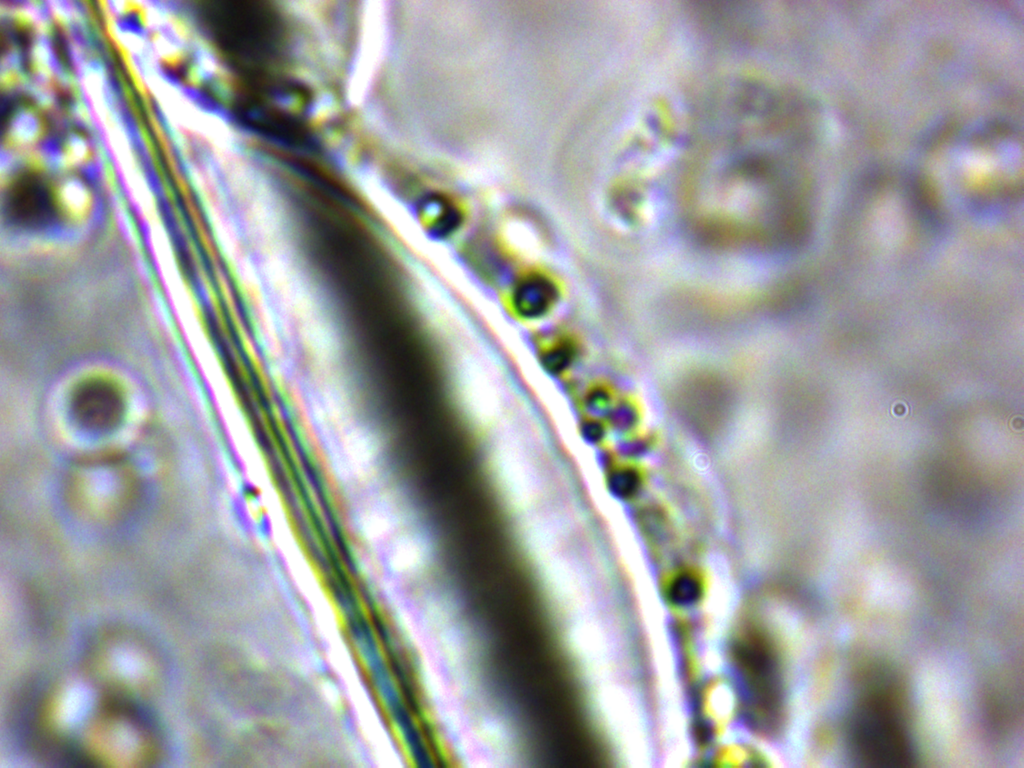
\includegraphics[width = 0.4\textwidth]{../analysis/data/iii_zwiebel/bilder/1.png}
  \caption{Exemplarische CMOS-Aufnahme der Zwiebelzelle.}
  \label{fig: zwiebelzelle}
\end{figure}

In dem Video 1.avi im Zwiebel-Anhang lässt sich beobachten, dass die Strukturen innerhalb der Zelle mit der optischen Pinzette
beeinflussen lassen. Innerhalb einer Mikrofaser können einzelne Vesikel gefangen werden und durch die Faser transportiert werden
(siehe Video 2.avi). Hierbei ist zu bobachten, dass die Kraft durch die Falle teilweise schwächer ist als die Kraft, die die
Vesikel in der Faser hält (Video 3.avi oder 4.avi). ach einer Auslenkung bewegen sich die Fasern wieder in eine
Ruhelage. Mit einem Laserstrom von $\SI{70}{\milli\ampere}$, was in etwa einer Fallensteifigkeit von
$\SI{26.2e-7}{\newton\per\meter}$ entspricht ist es nicht möglich ein Vesikel aus der Faser zu lösen (Video 70mA.avi). Mit einem STrom
von $\SI{170}{\milli\ampere}$ bzw. einer Fallensteifigkeit von $\SI{70e-7}{\newton\meter}$ gelingt dies (Video 170mA.avi).  

Abschließend soll die Geschwindigkeit der Vesikel bestimmt werden. Hierzu ist zunächst die Größe der Objekte relevant.
In Abbildung~\ref{fig: vesikel_size} ist eine Kameraaufnahme mit mehreren Vesikeln zu sehen. Hieraus wurden die Radien in Pixeln
bestimmt (siehe rote Kreise in der Abbildung). Im Mittel haben die Vesikel einen Radius von $\num{11.2}$ Pixeln. Im Vergleich hierzu haben die Quarzkugeln (siehe etwa
Abbildung~\ref{fig: quarz_screenshot}) einen Radius von ca. $\num{24.2}$ Pixeln. Aus der Kenntnis der Quarzkugelgöße von ca. $\SI{2}{\micro\meter}$
wird somit die Vesikelgröße zu
\begin{equation}
d_{\text{Vesikel}} \approx \SI{0.9}{\micro\meter}
\end{equation}
abgeschätzt.
Abbildung~\ref{fig: velocity} zeigt den Verlauf einer Messung währen sich ein Vesikel durh den Laserstrahl bewegt hat. Die temporäre
Auslenkung aus einem konstanten Wert ist deutlich zu erkennen. Aus dem Vesikeldurchmesser und dem zeitlichen Abstand der beiden vertikalen
Linien in Abbildung~\ref{fig: velocity} wird die Geschwindigeit berechnet
\begin{equation}
  v_{\text{Vesikel}} \approx \SI{1.03}{\micro\meter\per\second}.
\end{equation}
\begin{figure}
  \centering
  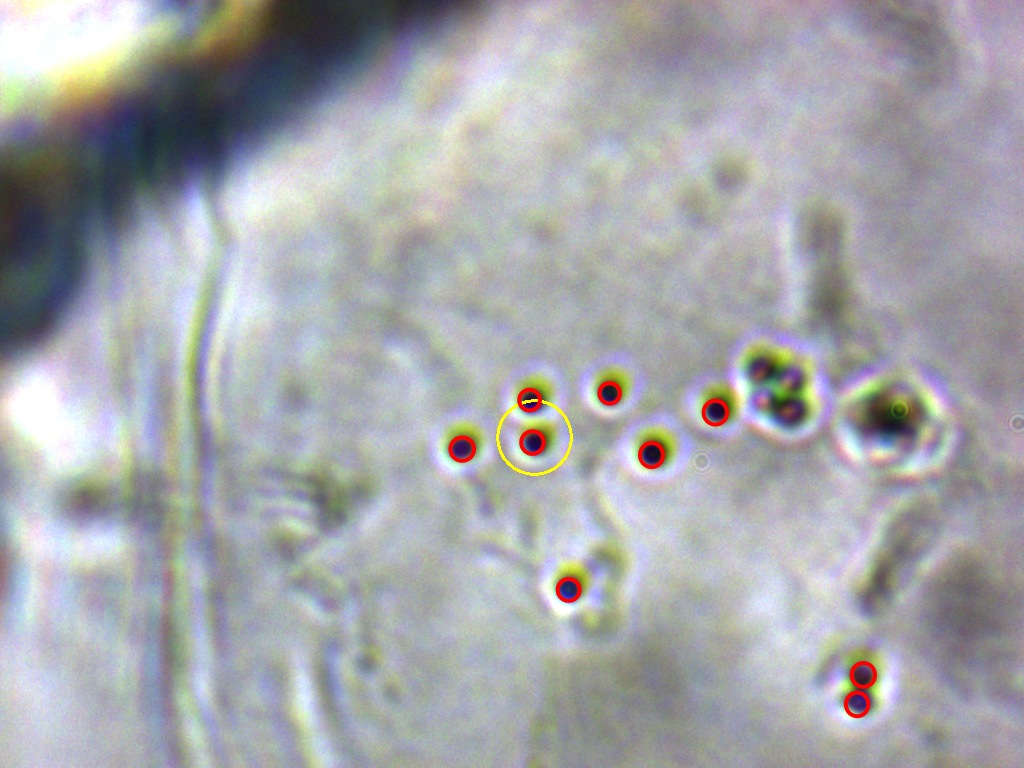
\includegraphics[width = 0.4\textwidth]{../analysis/data/iii_zwiebel/bilder/particle_size_(2)_circles.png}
  \caption{Aufnahme mehrerer Vesikel zur Abschätzung des Durchmessers. In rot sind die Kreise eingzeichnet, mit denen
  die Durchmesser abgeschätzt wurden. }
  \label{fig: vesikel_size}
\end{figure}
\begin{figure}
  \centering
  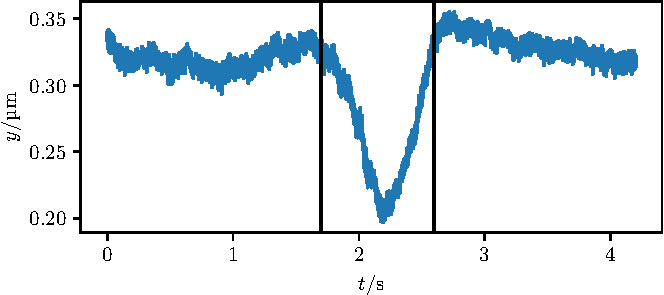
\includegraphics[scale = 1]{../analysis/data/iii_zwiebel/velocity/velocity.pdf}
  \caption{Gemessener zeitlicher Verlauf des Photodiodensignals beim Durchgang eines Vesikels durch den Laser.}
  \label{fig: velocity}
\end{figure}
